\documentclass[12pt]{beamer}
\usetheme{Copenhagen}
\definecolor{myblue}{rgb}{0,0.19,0.33}
\usecolortheme[named=myblue]{structure}
\usepackage[utf8]{inputenc}
\usepackage[serbian]{babel}
\usepackage{amsmath}
\usepackage{amsfonts}
\usepackage{amssymb}
\usepackage{multicol}
\usepackage{graphicx}
\usepackage{listings}
\author{Nikola Janković}
\title{Klasterovanje FIFA19}
\subtitle{Seminarski rad na kursu Istraživanje podataka 1}

\usepackage{xcolor}
 
\definecolor{codegreen}{rgb}{0,0.6,0}
\definecolor{codegray}{rgb}{0.5,0.5,0.5}
\definecolor{codepurple}{rgb}{0.58,0,0.82}
\definecolor{backcolour}{rgb}{0.95,0.95,0.92}
 
\lstdefinestyle{mystyle}{
    backgroundcolor=\color{backcolour},   
    commentstyle=\color{codegreen},
    keywordstyle=\color{magenta},
    numberstyle=\tiny\color{codegray},
    stringstyle=\color{codepurple},
    basicstyle=\ttfamily\footnotesize,
    breakatwhitespace=false,         
    breaklines=true,                 
    captionpos=b,                    
    keepspaces=true,                 
    numbers=left,                    
    numbersep=5pt,                  
    showspaces=false,                
    showstringspaces=false,
    showtabs=false,                  
    tabsize=2
}
 
\lstset{style=mystyle}


%\setbeamercovered{transparent=10} 
%\setbeamertemplate{navigation symbols}{} 
%\logo{} 
\institute{Matematički fakultet, Univerzitet u Beogradu} 
%\date{} 
%\subject{Istraživanje podataka 1} 
\begin{document}

\begin{frame}
\titlepage
\end{frame}

\section[Sadržaj]{}
\begin{frame}{Sadržaj}
\tableofcontents
\end{frame}

\section{Uvod}
\subsection{Motivacija}
\begin{frame}{Motivacija}
\begin{itemize}
\item Da li postoji povezanost između 
pozicije i kvaliteta fudbalera u stvarnom svetu
sa procenama koje su napravili kreatori igre
FIFA19 \pause
\item Popularnost ove oblasti. \pause
\item Autorova lična satisfakcija.
\end{itemize}
\end{frame}



\subsection{Skup podataka}
\begin{frame}{Skup podataka}
\begin{itemize}
\onslide<1-> {
\item 18000 slogova 
\item 89 atributa
}
\end{itemize} 
\onslide<2-> {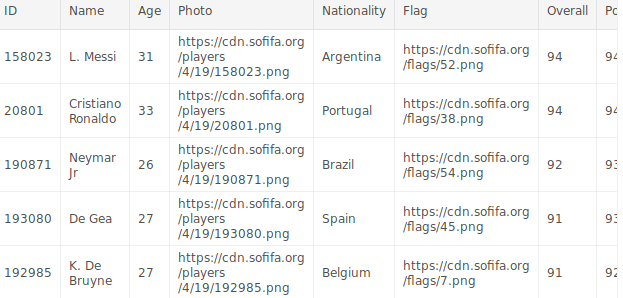
\includegraphics[scale=0.4]{../head}
}

\end{frame}

\begin{frame}{Skup podataka}
\begin{table}
\scriptsize
\begin{tabular}{c | c | c | c | c | c | c | c | c}
 & Age & Overall & Potential & Special 
& Int. Reput. & Weak Foot & Skill 
Moves \\
\hline
\hline
mean & 25.12 & 62.24 & 71.31 & 1597.81 & 1.11 &
2.95 & 2.36 \\
std & 4.67 & 6.9 & 6.13 & 272.59 & 0.39 &
0.66 & 0.75 \\
min & 16 & 46 & 48 & 731 & 1 & 1 & 1 \\
25\% & 21 & 62 & 67 & 1457 & 1 & 3 & 2 \\
50\% & 25 & 66 & 71 & 1635 & 1 & 3 & 2 \\
75\% & 28 & 71 & 75 & 1787 & 1 & 3 & 3 \\
max & 45 & 94 & 95 & 2346 & 5 & 5 & 5 \\
\end{tabular}
\end{table}
\end{frame}


\begin{frame}{Skup podataka}
\begin{itemize}
\item<1-> \emph{Value}
\item<2-> \emph{International reputation}
\item<3-> \emph{Loaned From}
\item<4-> \emph{LS, ST, RS, ..., RB}
\item<5-> \emph{Release Clause}
\end{itemize}
\end{frame}



\section{Analiza podataka}
\subsection{Statistike}
\begin{frame}{Statistike}
\begin{figure}
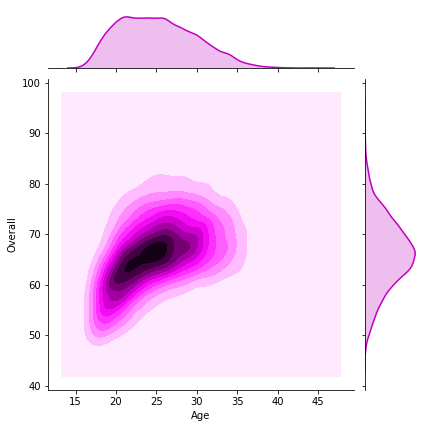
\includegraphics[scale=0.4]{../stat1}
\caption{Overall $\sim$ Age}
\end{figure}
\end{frame}

\begin{frame}{Statistike}
\begin{figure}
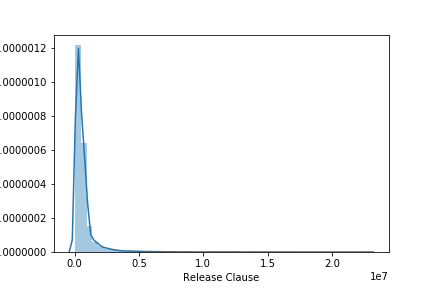
\includegraphics[scale=0.4]{../stat2}
\caption{Raspodela izlazne klauze}
\end{figure}
\end{frame}


\begin{frame}[t]{Statistike}
\begin{figure}
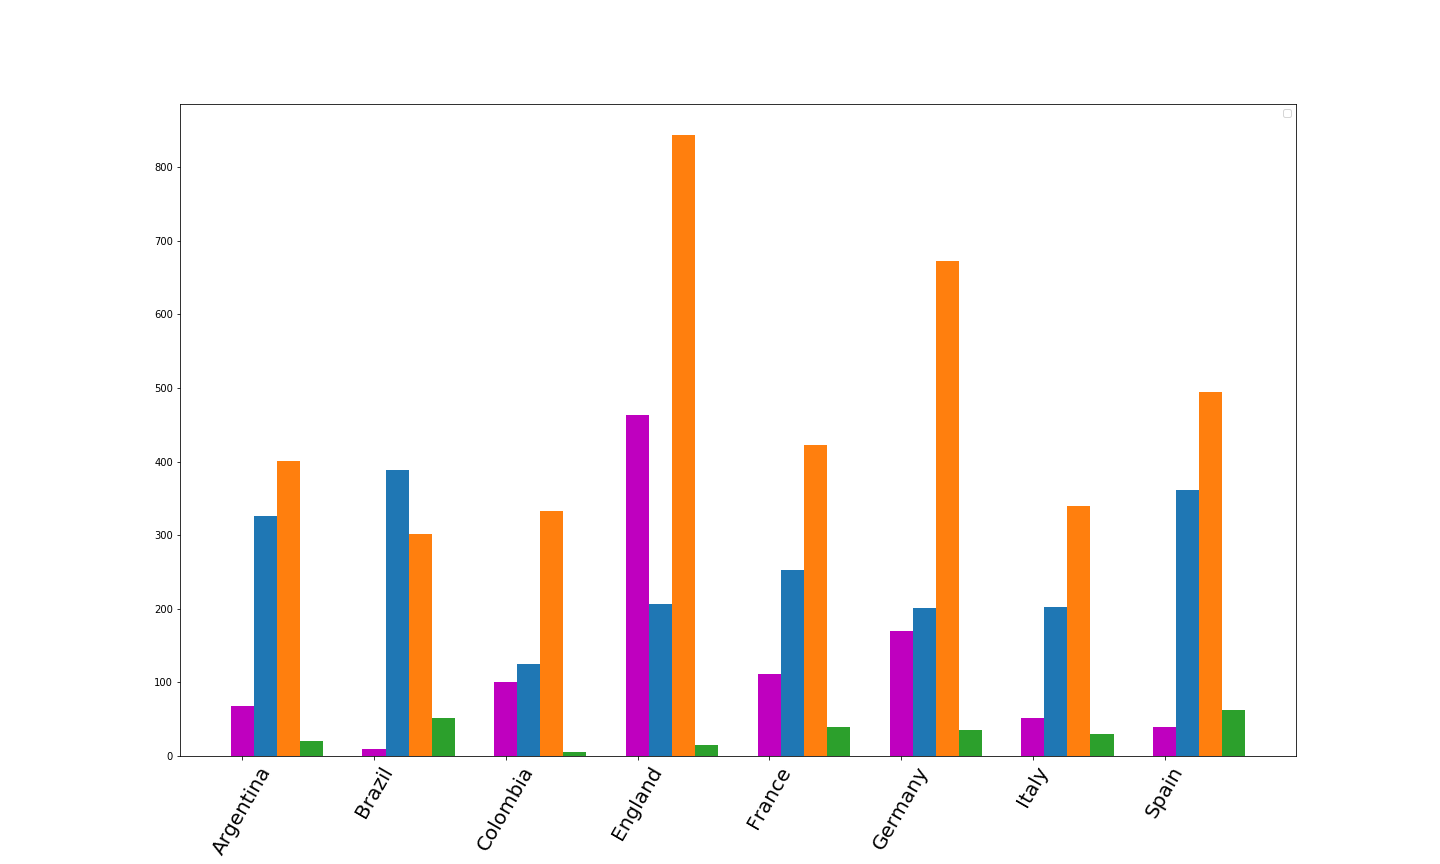
\includegraphics[scale=0.15]{../stat3} 

\end{figure}\pause
Zašto?
\end{frame}

\subsection{Pretprocesiranje}
\begin{frame}{Pretprocesiranje}
\begin{itemize}
\item
ID, Name,
Photo, Club, Club Logo, Flag, Jersey Number, Loaned From, Work Rate,
Real Face, Joined, Body Type \pause
\item LS, ST, RS, ..., RB \pause
\item Wage, Value, Release Clause \pause
\item Country
\end{itemize}
\end{frame}


\section{Primena algoritama}
\begin{frame}{Primena algoritama}
\begin{itemize}
\item Na kursu
\begin{itemize}
\item K-means
\item DBSCAN
\item Self Organizing Map
\item Hijerahijsko klasterovanje
\end{itemize}
\item Dodatno
\begin{itemize}
\item Meanshift
\item BIRCH
\end{itemize}
\end{itemize}

\end{frame}

\subsection{K-means}
\begin{frame}{K-means}
\begin{figure}
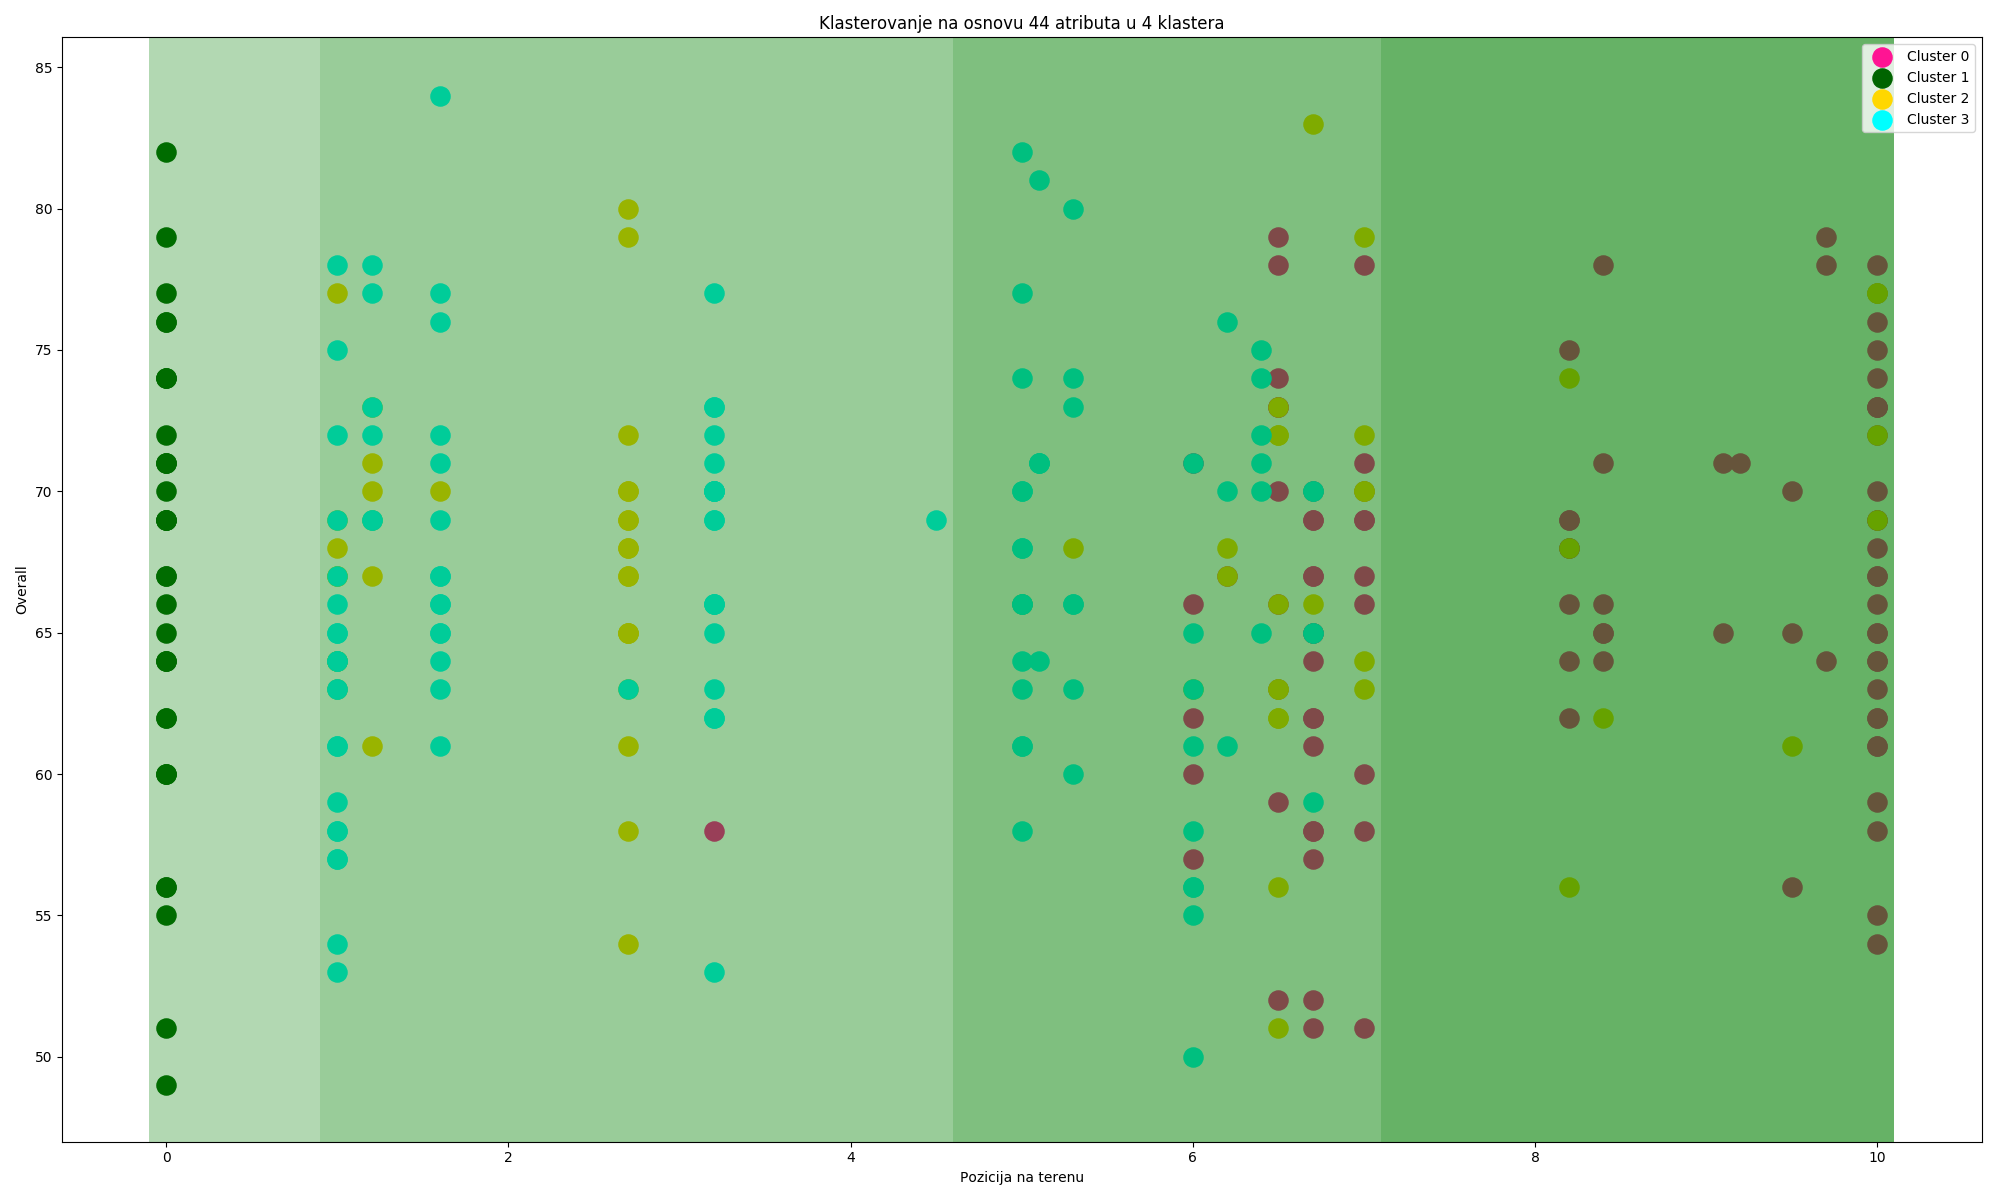
\includegraphics[scale=0.2]{../position_clustering}
\end{figure}
\end{frame}

\begin{frame}{K-means}
\begin{figure}
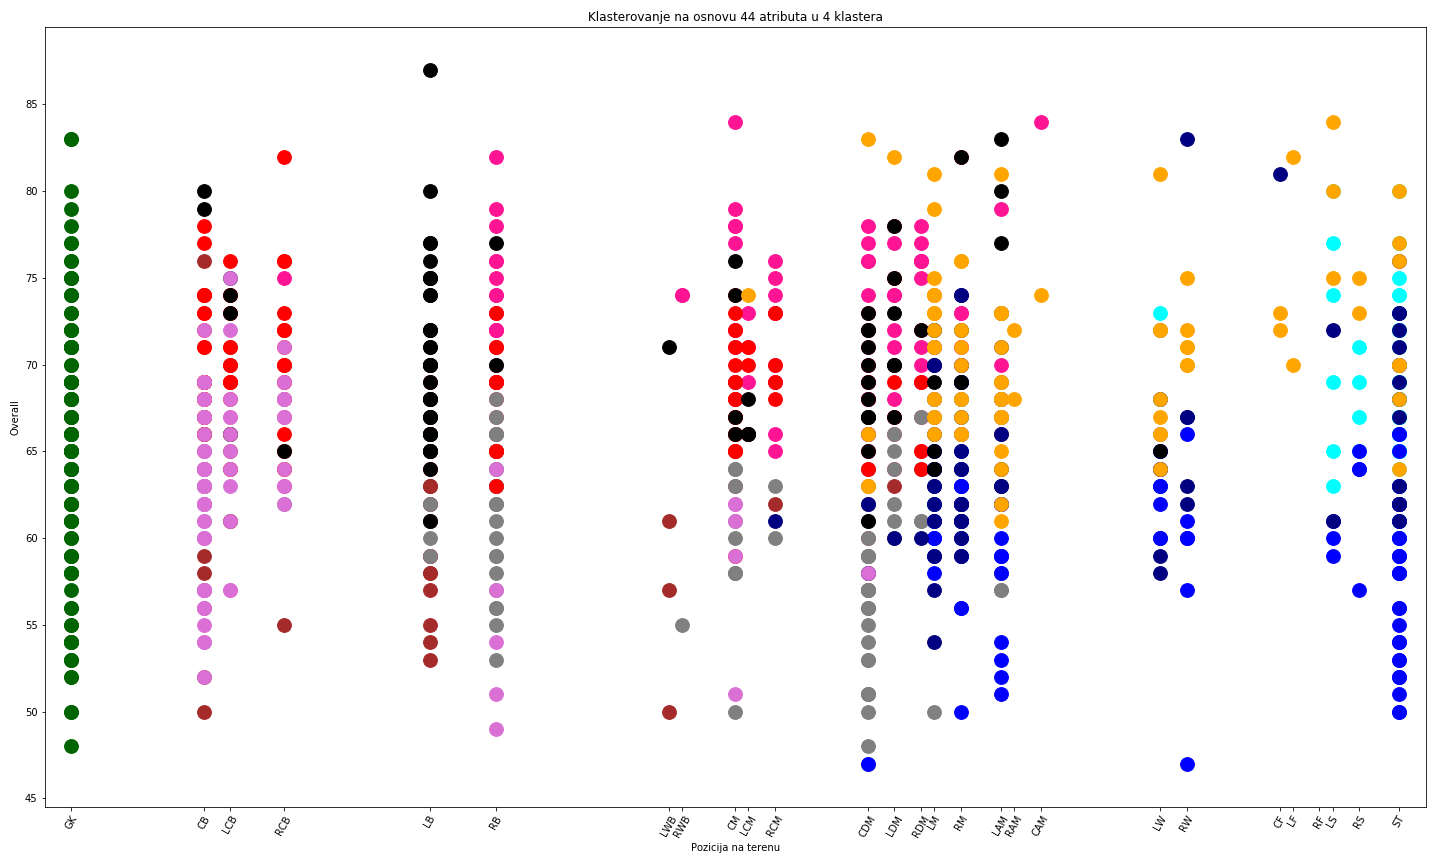
\includegraphics[scale=0.15]{../kmeans_11}
\end{figure}
Senka koeficijent dobijen ovakvim klasterovanjem je 0.176189407.
\end{frame}

\subsection{DBSCAN}
\begin{frame}{DBSCAN}
\begin{multicols}{2}

\begin{table}
\scriptsize
\begin{tabular}{c|c|c}
EPS & MIN\_SAMPLE & SENKA KOEF. \\
\hline
\hline

0.2 & 15 & 0.1869359\\
0.2 & 17 & -0.167595\\
0.2 & 19 & -0.217335\\
0.2 & 22 & -0.119365\\
0.2 & 25 & -0.110591\\

0.25 & 15 & 0.02033613\\
0.25 & 17 & -0.0788248\\
0.25 & 19 & -0.0136990\\
0.25 & 22 & 0.08744345\\
0.25 & 25 & -0.0008812\\

0.28 & 15 & 0.1888508\\
0.28 & 17 & 0.1003213\\
0.28 & 19 & 0.1004942\\
0.28 & 22 & 0.0512825\\
0.28 & 25 & 0.1040002\\
\end{tabular}
\end{table}


\begin{table}
\scriptsize
\begin{tabular}{c|c|c}
EPS & MIN\_SAMPLE & SENKA KOEF. \\
\hline
\hline

0.3 & 15 & 0.2102658\\
0.3 & 17 & 0.0920832\\
0.3 & 19 & 0.2000161\\
0.3 & 22 & 0.1222602\\
0.3 & 25 & 0.1196769\\


\textbf{0.35} & \textbf{15} & \textbf{0.2683946}\\
0.35 & 17 & 0.2625584\\
0.35 & 19 & 0.2588889\\
0.35 & 22 & 0.2474575\\
0.35 & 25 & 0.1936369\\

\end{tabular}
\end{table}
\end{multicols}
\end{frame}


\begin{frame}{DBSCAN}
\begin{figure}
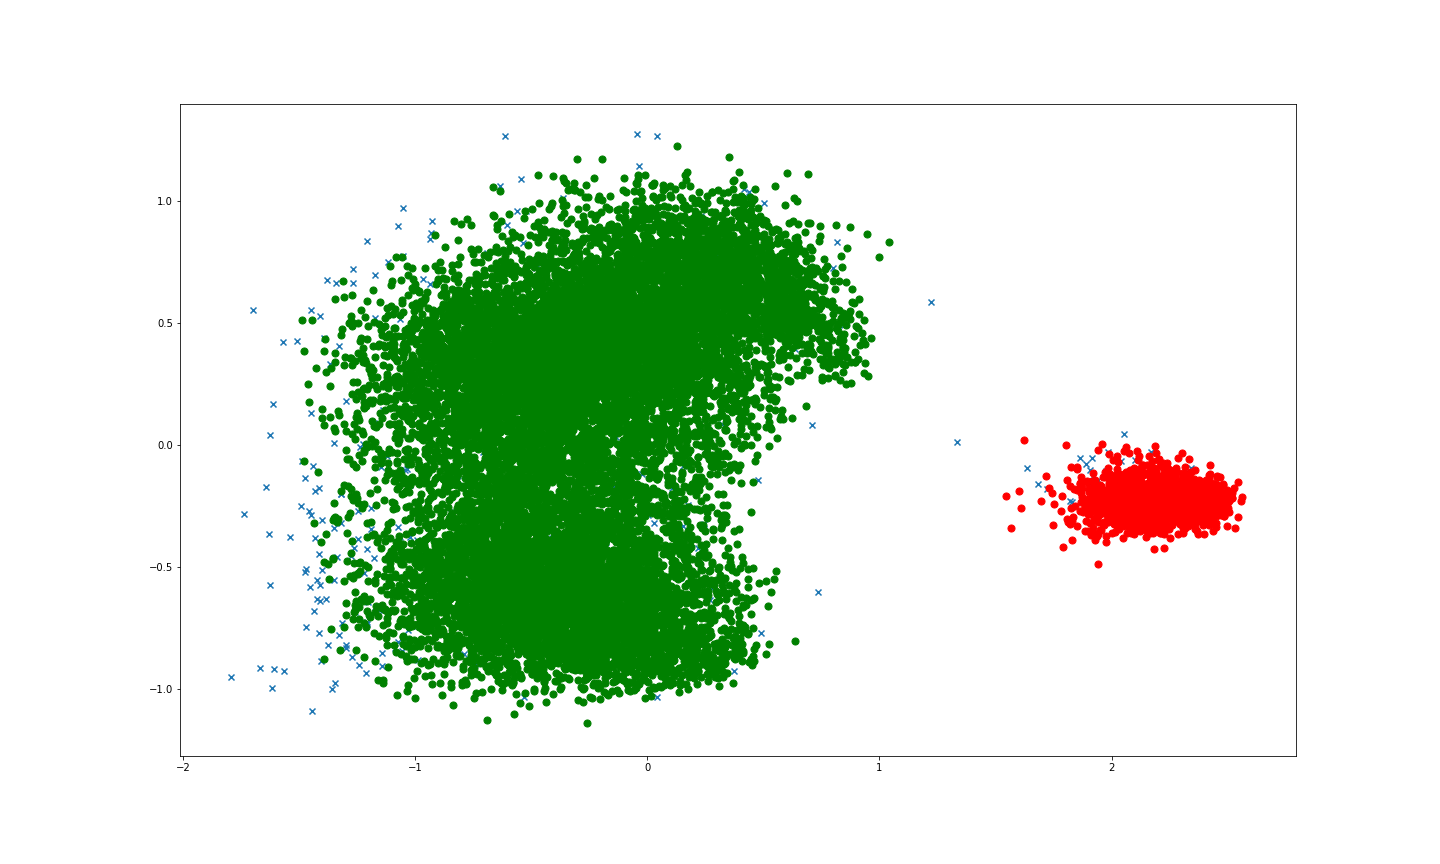
\includegraphics[scale=0.2]{../dbscan_pca_035_15}\vspace*{-10mm}
\caption{DBSCAN pca}
\end{figure}
\end{frame}

\subsection{Self Organizing Map}
\begin{frame}{SOM}
\begin{figure}
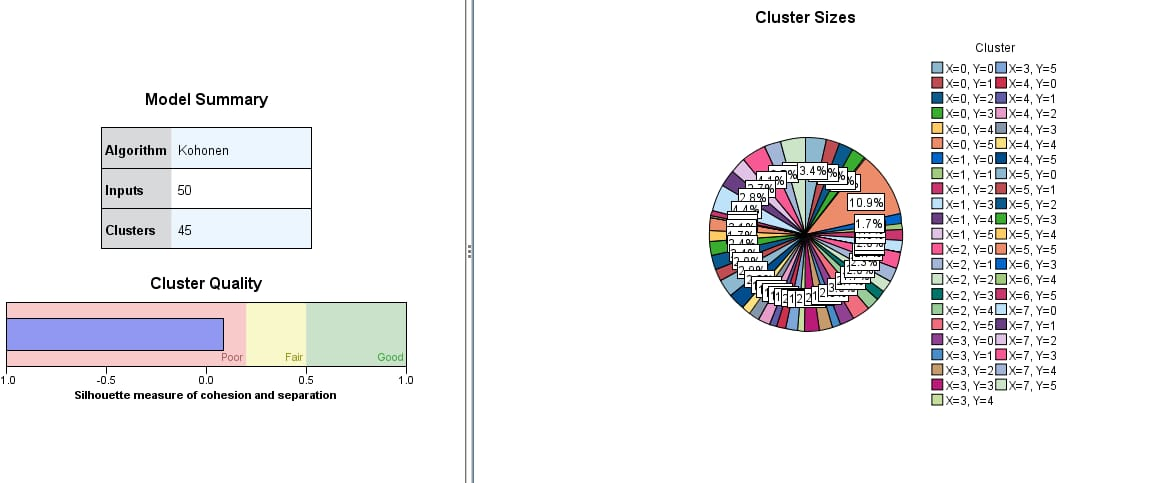
\includegraphics[scale=0.3]{../kohonen_spss.png}
\end{figure}
\end{frame}

\begin{frame}{SOM}
\begin{figure}
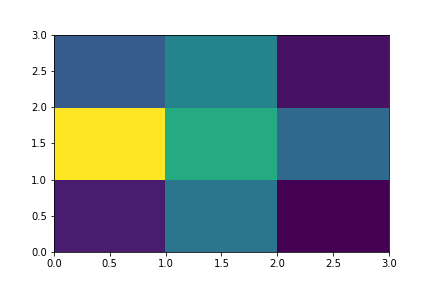
\includegraphics[scale=0.2]{../distance_map_som}
\end{figure}

\begin{figure}
\fbox{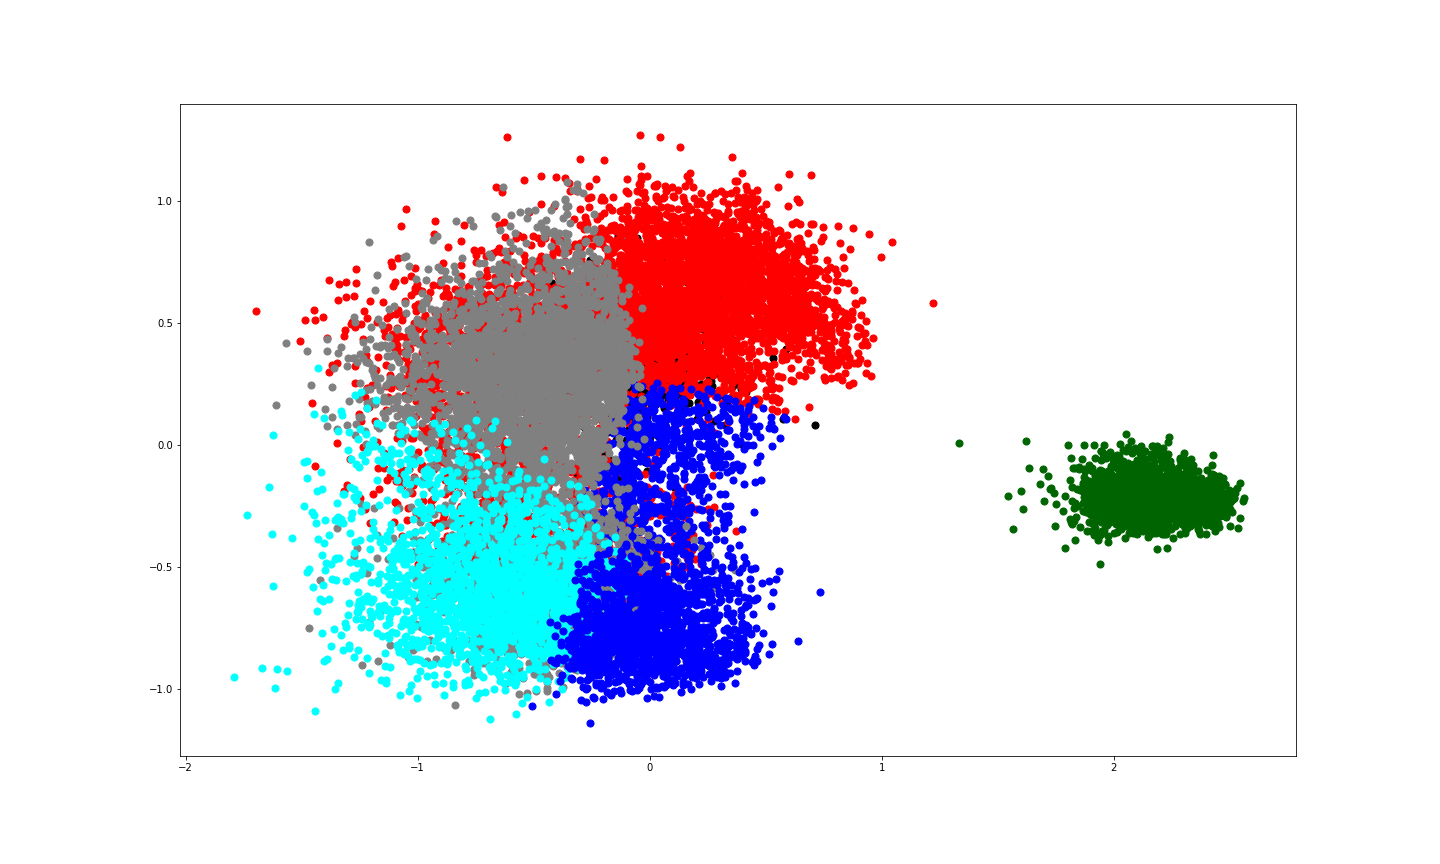
\includegraphics[scale=0.15]{../som_pca5}}
\end{figure}
\end{frame}


\subsection{Hijerarhijsko klasterovanje}
\begin{frame}[t]{Hijerarhijsko klasterovanje}
Primećeno je da najbolji senka koeficijent za
3-7 klastera
daje \emph{single} veza. Pa je za tu vezu isproban algoritam za 11 klastera 

\begin{figure}
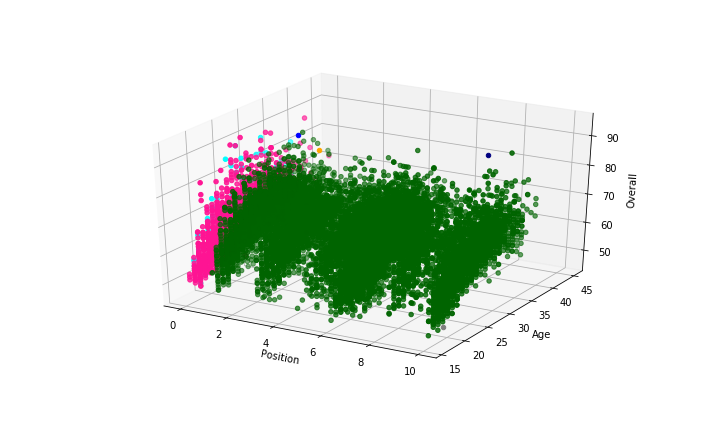
\includegraphics[scale=0.3]{../agglomerative_11_3d_overall_age_position}
\end{figure}

\end{frame}

\begin{frame}
\begin{figure}
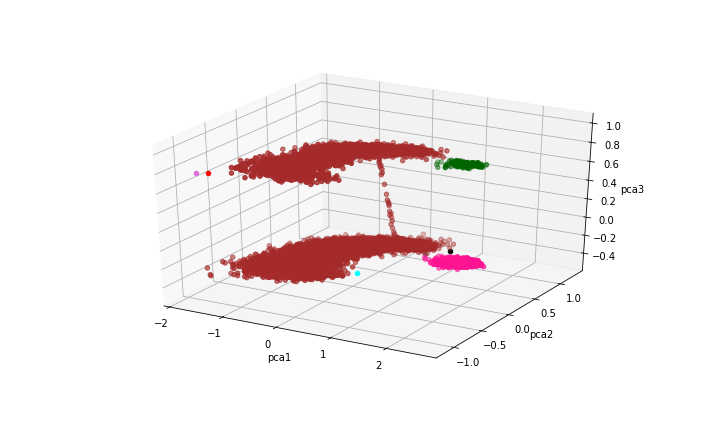
\includegraphics[scale=0.4]{../agglomerative_11_pca_3d}
\end{figure}
\end{frame}

\subsection{Meanshift}
\begin{frame}[fragile]{Meanshift}
\begin{lstlisting}[language=Pascal, basicstyle=\scriptsize]
Input: bandwith, skup podataka
WHILE postoji objekat koji nije dodeljen nijednom klasteru DO :
	izaberi jedan od nedodeljenih objekata i oznaci
	da pripada novom klasteru
	REPEAT:
	azuriraj srednju tacku ( centroid ) u trenutnom klasteru ;
	sve tacke koje se nalaze na razdaljini manjoj
	od bandwidth oznaci ih da pripadaju trenutnom
	klasteru;
	UNTIL postoji promena na trenutnom klasteru
\end{lstlisting}

\end{frame}


\begin{frame}{Meanshift}
\begin{itemize}
\item Bandwith izabran 1.5 uz pomoć
\emph{sklearn.estimate\_bandwith()} \pause
\item Odličan senka koeficijent, ali samo 2 klastera. \pause
\item Smanjen bandwith na 0.5.\pause
\item Dobijena 4 klastera, senka koeficijent i dalje preko 0.5
\end{itemize}
\end{frame}

\begin{frame}{Meanshift}
\begin{figure}
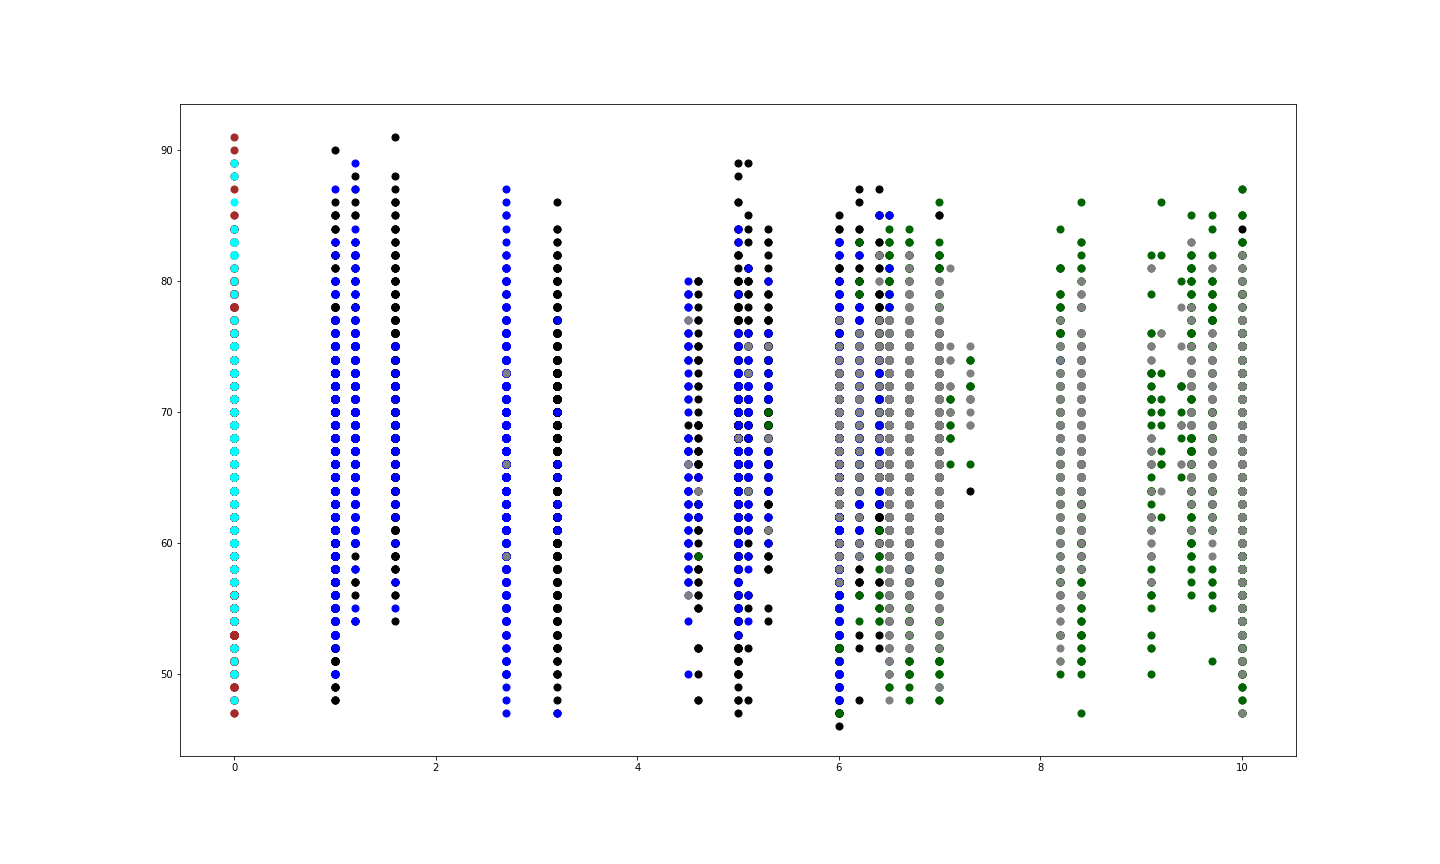
\includegraphics[scale=0.15]{../meanshift_bandwith05}
\end{figure}
\end{frame}


\subsection{BIRCH}
\begin{frame}[t]{BIRCH}
\footnotesize
\begin{definition} 
BIRCH - ( balanced iterative reducing and clustering using hierarchies)
Hibridni algoritam za klasteorvanje koji se zasniva na pravljenju CF(Clusters
Features)-stabla.
\end{definition}
Za k=11 senka koeficijent = 0.61
\begin{figure}
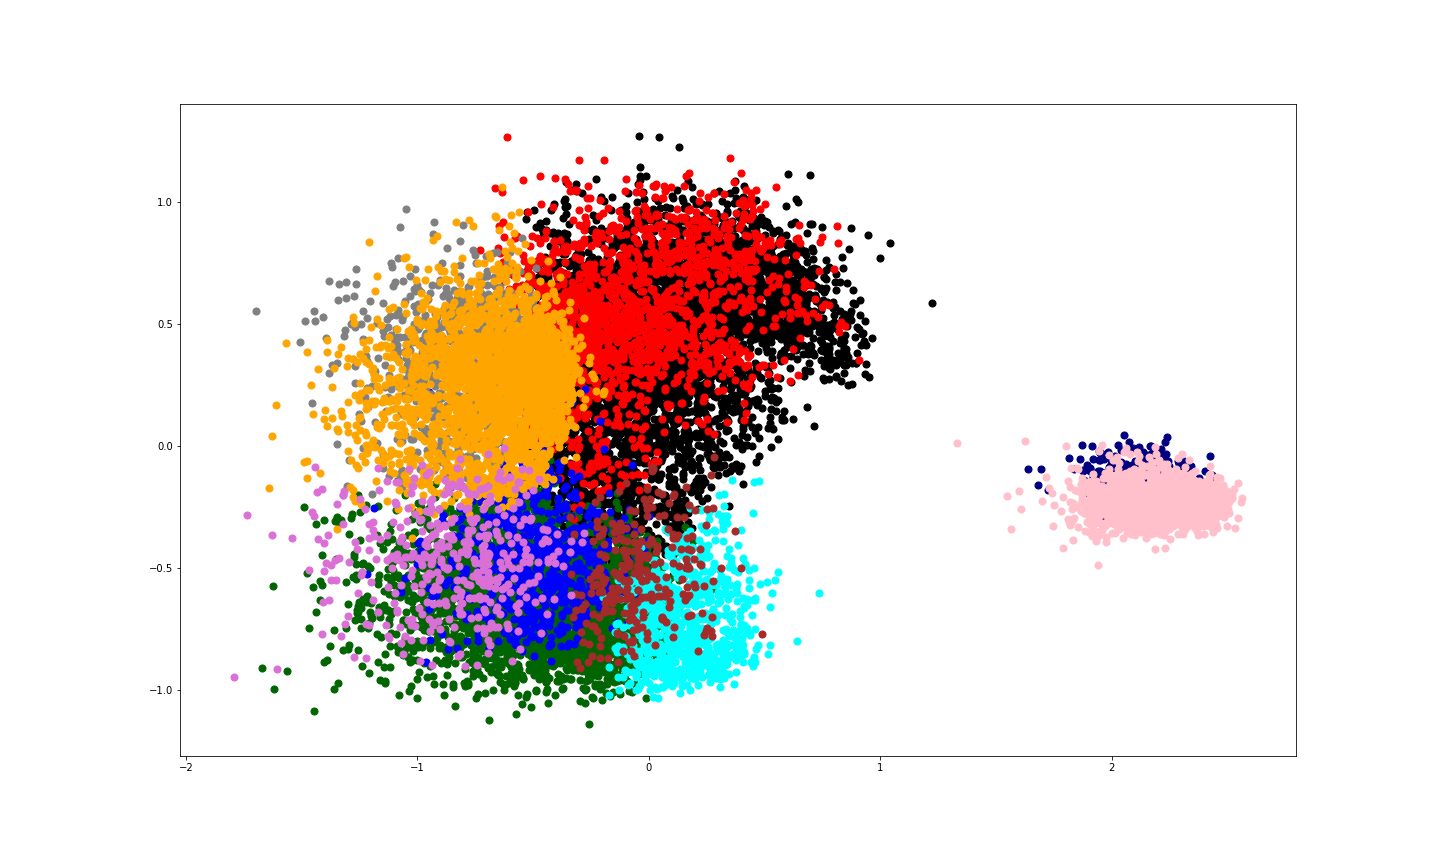
\includegraphics[scale=0.1]{../birch_11_pca}
\end{figure}
\end{frame}

\section{Zaključak}
\begin{frame}{Zaključak}
\begin{itemize}
\item Koji se algoritam najbolje pokazao? \pause
\item Dalje mogućnosti sa ovim skupom? \pause
\item Pitanja?
\end{itemize}

\end{frame}
\end{document}

